\chapter{تنظيم ضغط الدم والجهد}\label{ch:b2:blood-pressure}

انهض سريعًا بعد اضطجاع، فينزح في ثانية واحدة نصف لتر من
الدم إلى أوردة ساقيك؛ \omterm{def:b2:heart:anatomy}{فالقلب}، إذ يتلقى أقل، يضخ أقل،
ويهبط الضغط عند الرأس، ويصير الدماغ --- وهو على \qty{40}{cm} فوق
\omterm{def:b2:heart:anatomy}{القلب} ولا يستطيع خزن الأكسجين --- على ثانية أو
ثانيتين من الغشي. لكنه لا يفعل إلا نادرًا، لأن منعكسًا قد
شدّ \omterm{def:b2:blood-circulation:vessels}{الشرينات} وسرّع \omterm{def:b2:heart:anatomy}{القلب} في غضون نبضة واحدة. واعدُ خلف
حافلة، فتحتاج العضلات عشرة أمثال ما كان لها من دم في الراحة؛
وتناله في غضون دقيقة، ويبقى الضغط الذي يسوقه
ثابتًا في حين تهبط مقاومة الجسم كله بمقدار
الثلثين. وهذا الفصل في ذلك التنظيم: ما الذي يقرر
الضغط، وكيف يُستشعر، والمنعكس السريع والهرمونات البطيئة
التي تصححه، وكيف يعاد تنظيم الجملة، لا تُتجاوز،
في الجهد.

\section{ماهية الضغط}

\begin{theorem}[معادلة الدوران]\label{thm:b2:blood-pressure:equation}
\index{ضغط شرياني متوسط}\index{مقاومة محيطية كلية}
\omterm{thm:b2:blood-pressure:equation}{الضغط الشرياني المتوسط} $\bar P$ هو جداء ما يدفعه \omterm{def:b2:heart:anatomy}{القلب}
في ما تمانعه الأوعية:
\[
\bar P - P_{\text{وريدي}} = Q\,R, \qquad Q = f\times V_s,
\]
حيث $Q$ \omterm{thm:b2:heart:starling}{النتاج القلبي} (أي معدل \omterm{def:b2:heart:anatomy}{القلب} $f$ في \omterm{prop:b2:heart:cycle}{حجم الضربة}
$V_s$)، و$R$ \omterm{thm:b2:blood-pressure:equation}{المقاومة المحيطية الكلية} --- أي \omterm{def:b2:blood-circulation:vessels}{شرينات} كل
الأعضاء على التوازي --- و$P_{\text{وريدي}}$ الضغط الوريدي،
وهو قريب من الصفر. وفي الراحة يعطي $\qty{5}{L/min}\times\qty{1.08}{mmHg.s/mL}$
\qty{90}{mmHg}. وكل تنظيم للضغط يفعل في واحد من ثلاثة
مقادير: المعدل، أو \omterm{prop:b2:heart:cycle}{حجم الضربة} (عبر الامتلاء والقابلية
للانقباض في \cref{ch:b2:heart})، أو المقاومة (عبر
نصف قطر \omterm{def:b2:blood-circulation:vessels}{الشرينات}، مرفوعًا إلى القوة الرابعة). ولأن الأعضاء على
التوازي، يكون الجريان إلى كل منها حصته من الضغط مقسومةً على
مقاومته الخاصة: فتوسيع \omterm{def:b2:blood-circulation:vessels}{شرينات} عضو واحد يرفع
جريانه دون تغيير جريان غيره، ما دام الضغط ثابتًا ---
وإبقاء الضغط ثابتًا هو غاية التنظيم.
\end{theorem}
\begin{proof}
قانون أوم لمائع: الجريان عبر مقاومة هو هبوط الضغط
عليها مقسومًا على المقاومة (بوازوي،
\cref{ch:b2:blood-circulation})؛ وللمقاومات على التوازي
تتجمع الجريانات ويكون $1/R = \sum 1/R_i$. والضغط المتوسط على مدى نبضة
يقارب الانبساطي زائدًا ثلث \omterm{thm:b2:blood-circulation:windkessel}{ضغط النبض}:
$80 + 40/3 = \qty{93}{mmHg}$.
\end{proof}

\begin{omfigure}
\begin{tikzpicture}[every node/.style={font=\scriptsize}, >=stealth]
  \node[draw, rounded corners, fill=omThm!15, minimum width=2.4cm, minimum height=1cm, align=center] (heart) at (0,0) {القلب\\$Q = f\,V_s$};
  \draw[very thick, omThm] (1.2,0) -- (2.4,0);
  \draw[very thick, omThm] (2.4,-2.4) -- (2.4,2.4);
  \foreach \y/\org/\r in {2.0/{الدماغ}/{$R_1$}, 1.0/{عضلة القلب}/{$R_2$}, 0/{الأمعاء والكبد}/{$R_3$}, -1.0/{الكليتان}/{$R_4$}, -2.0/{العضلات والجلد}/{$R_5$}} {
    \draw[very thick, omThm] (2.4,\y) -- (3.6,\y);
    \draw[thick, decorate, decoration={zigzag, segment length=4pt, amplitude=2pt}] (3.6,\y) -- (5.0,\y);
    \node[above] at (4.3,\y+0.05) {\org};
    \node[below] at (4.3,\y-0.05) {\r};
    \draw[very thick, omDef] (5.0,\y) -- (6.2,\y);
  }
  \draw[very thick, omDef] (6.2,-2.4) -- (6.2,2.4);
  \draw[very thick, omDef] (6.2,0) -- (7.4,0) |- (0,-3.2) -- (0,-0.5);
  \node[omThm, above] at (1.8,0.05) {$\bar P$};
  \node[omDef, below] at (3.7,-3.2) {أوردة، $P_{\text{وريدي}} \approx 0$};
  \node[anchor=west, align=left] at (7.8,1.5) {الأعضاء على التوازي:\\$1/R = \sum 1/R_i$\\الجريان إلى العضو $i$: $\bar P/R_i$};
\end{tikzpicture}

{\small الدوران دارةً كهربائية: مضخة واحدة، وضغط واحد،
ومقاومات \omterm{def:b2:blood-circulation:vessels}{شرينات} الأعضاء على التوازي. فيأخذ كل عضو
$\bar P/R_i$؛ والتنظيم يبقي $\bar P$ ثابتًا بينما تُعدَّل $R_i$
على قدر الطلب.}
\end{omfigure}

\begin{proposition}[لماذا يجب تنظيم الضغط]\label{prop:b2:blood-pressure:why}
فإن هبط كثيرًا لم يُروَ الدماغ --- وهو على \qty{40}{cm} فوق \omterm{def:b2:heart:anatomy}{القلب} في
بالغ واقف، وذلك يكلف \qty{31}{mmHg} من العمود الهيدروستاتي ---
ولا عضلة \omterm{def:b2:heart:anatomy}{القلب} نفسها: ويخفق الدماغ في غضون
ثوانٍ. وإن ارتفع كثيرًا تضررت الأوعية: فيثخن الجدار
الشرياني ويجسأ، وتتندب كبيبات الكلية، وتنزف
الشبكية، ويكدح \omterm{def:b2:heart:anatomy}{القلب} ضد الضغط حتى يخفق.
وعلى الضغط أيضًا أن يبقى ثابتًا في حين تتغير طلبات الأعضاء
برتبة مقدار كاملة --- الأمعاء بعد وجبة، والعضلات
في الجهد، والجلد في الحر --- وفي حين يُفقد حجم الدم نفسه
في نزف أو عرق. ويقوم بذلك جهازان: منعكس
عصبي يفعل في غضون نبضة في المعدل \omterm{prop:b2:heart:cycle}{وحجم الضربة}
والمقاومة، وجمل هرمونية تفعل على مدى ساعات وأيام
في المقاومة، وقبل كل شيء في حجم الدم عبر
الكلية.
\end{proposition}

\begin{omfigure}
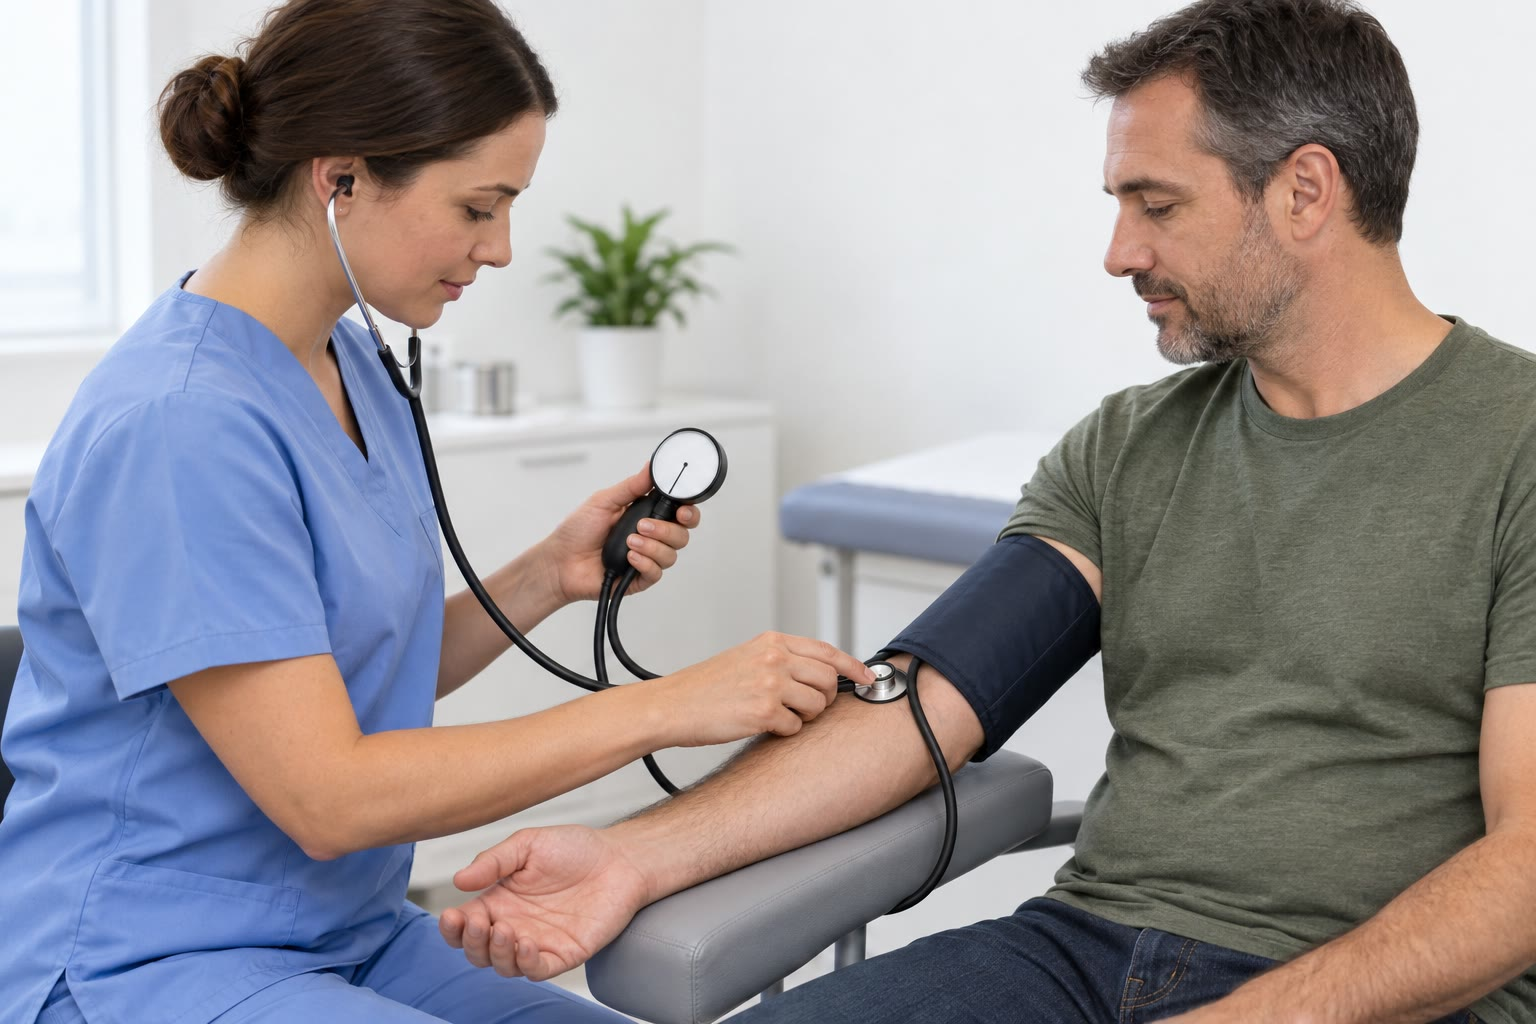
\includegraphics[width=0.6\linewidth]{images/book4/ai/b4-18-blood-pressure-cuff.jpg}

{\small قياس الضغط. تُنفخ الكمّامة فوق الضغط
الانقباضي حتى لا يمر دم؛ وإذ تُرخى، تدل أول أصوات
الجريان المضطرب تحت السماعة على الضغط
الانقباضي، ويدل زوالها، حين يبقى \omterm{def:b2:blood-circulation:vessels}{الشريان}
مفتوحًا طوال الدورة، على الانبساطي.}
\end{omfigure}

\section{الحلقة السريعة: المنعكس الضغطي}

\begin{definition}[المنعكس الضغطي]\label{def:b2:blood-pressure:baroreflex}
\index{مستقبل ضغط}\index{منعكس ضغطي}\index{مركز حركي وعائي}\index{جملة عصبية ذاتية}
مستقبلات التمدد في جدر الجيبين السباتيين (عند مفترق
كل \omterm{def:b2:blood-circulation:vessels}{شريان} سباتي، تحت الفك) وفي قوس الأبهر --- وهي
\emph{مستقبلات الضغط} --- تنطلق بمعدل يرتفع مع الضغط
الذي يمططها، وأسرع كلما كان الضغط صاعدًا. وتبلغ أعصابها
\emph{المراكز القلبية الوعائية} في البصلة السيسائية، وهي
تتحكم في فرعي الصادر الذاتي: المبهم، الذي يبطئ
الأستيل كولين الذي يطلقه العقدةَ الجيبية الأذينية، والأعصاب
الودّية، التي يسرّع النورأدرينالين الذي تطلقه العقدةَ، ويقوّي
\omterm{def:b2:heart:anatomy}{البطين}، ويقبض \omterm{def:b2:blood-circulation:vessels}{الشرينات} (فيرفع $R$)، ويقبض
الأوردة (فيعصر الدم المخزون نحو \omterm{def:b2:heart:anatomy}{القلب} ويرفع
الامتلاء). وارتفاع الضغط يزيد انطلاق مستقبلات الضغط، فيهيّج
المبهم ويثبط الصادر الودّي: فيهبط المعدل،
وترتخي \omterm{def:b2:blood-circulation:vessels}{الشرينات}، وينزل الضغط. والهبوط يفعل
العكس. والحلقة \emph{تغذية راجعة سالبة} ذات قيمة
مرجعية قرب \qty{95}{mmHg}، وتأخر نحو ثانية، وربح
يُصحَّح به أي اضطراب إلى حدود خُمس حجمه:
وهي السبب في أنك لا يُغشى عليك عند الوقوف.
\end{definition}
\begin{proof}[شواهد]
وجد هيرنغ (1923) أن الضغط على الجيب السباتي يبطئ
\omterm{def:b2:heart:anatomy}{القلب} ويخفض الضغط، وأن قطع عصب الجيب
يلغي الاستجابة. وإرواء جيب سباتي معزول عند ضغوط
معينة مع تسجيل الضغط الشرياني للحيوان أعطى
المنحني السيني للمنعكس: فضغط الحيوان يهبط كلما رُفع
ضغط الجيب، هبوطًا شديد الميل حول \qty{100}{mmHg} وقليلًا
خارج \qtyrange{60}{160}{mmHg}. والكلاب المقطوعة أعصاب جيوبها
وأبهرها تبقي ضغطًا متوسطًا سويًا على مدى أيام لكنه
شديد التقلب من دقيقة إلى أخرى --- فالمنعكس عازل، لا
مقرر للمستوى بعيد المدى.
\end{proof}

\begin{omfigure}
\begin{tikzpicture}[every node/.style={font=\scriptsize}, >=stealth]
  \node[draw, rounded corners, fill=omDef!15, align=center] (bp) at (0,0) {الضغط الشرياني\\$\bar P$};
  \node[draw, rounded corners, fill=omDef!15, align=center] (baro) at (4.2,0) {مستقبلات الضغط\\الجيب السباتي وقوس الأبهر\\معدل الانطلاق $\uparrow$ مع $\bar P$};
  \node[draw, rounded corners, fill=omProp!20, align=center] (med) at (8.6,0) {البصلة السيسائية:\\المراكز القلبية الوعائية};
  \node[draw, rounded corners, fill=omThm!15, align=center] (vag) at (8.6,-2.2) {المبهم $\uparrow$: المعدل $\downarrow$};
  \node[draw, rounded corners, fill=omThm!15, align=center] (sym) at (4.2,-2.2) {الودّي $\downarrow$: المعدل والقابلية للانقباض\\والمقوية الشرينية والوريدية $\downarrow$};
  \draw[->, thick] (bp) -- (baro); \draw[->, thick] (baro) -- (med);
  \draw[->, thick] (med) -- (vag); \draw[->, thick] (med) -- (sym);
  \draw[->, thick] (sym.west) -| (bp.south) node[pos=0.75, left, align=right] {$Q\downarrow$ و$R\downarrow$:\\$\bar P\downarrow$};
  \draw[->, thick] (vag.west) -- (sym.east);
  \node[anchor=north, align=center] at (4.3,-3.2) {ارتفاع الضغط يُجاب بهبوط: تغذية راجعة سالبة، وتأخر ثانية واحدة};
\end{tikzpicture}

{\small \omterm{def:b2:blood-pressure:baroreflex}{المنعكس الضغطي}. ارتفاع الضغط الشرياني يزيد
انطلاق مستقبلات الضغط، فيدفع البصلة إلى إبطاء \omterm{def:b2:heart:anatomy}{القلب}
وإرخاء الأوعية؛ والهبوط يفعل العكس.}
\end{omfigure}

\begin{theorem}[ربح حلقة التغذية الراجعة السالبة]\label{thm:b2:blood-pressure:gain}
\index{ربح التغذية الراجعة}
إذا كان اضطراب ما سيغير الضغط، لولا التنظيم، بمقدار
$\Delta P_0$، وكانت الحلقة تجيب أي انحراف $\Delta P$ بتصحيح
مقداره $-G\,\Delta P$ (وهو \emph{الربح المفتوح الحلقة} $G$)، فإن
الانحراف الباقي بعد فعل الحلقة هو
\[
\Delta P = \frac{\Delta P_0}{1 + G}.
\]
وللمنعكس الضغطي $G \approx 4$: فالوقوف، الذي كان سيُهبط
الضغط عند \omterm{def:b2:heart:anatomy}{القلب} نحو \qty{40}{mmHg}، يهبطه
\qty{8}{mmHg}؛ والنزف الذي كان سينصّف الضغط يخفضه
بمقدار العُشر --- إلى أن يتجاوز الفقد ما تستطيع أوعية أضيق \omterm{def:b2:heart:anatomy}{وقلب}
أسرع إخفاءه. فالمنعكس لا يلغي الاضطراب؛
بل يقسمه على خمسة. وهو \emph{يعيد ضبط نفسه}: فإذا أُبقي عند ضغط
جديد ساعات، تكيفت مستقبلات الضغط ودافعت عن المستوى الجديد، وهو
سبب عجز المنعكس عن شفاء فرط الضغط، وسبب كون المستوى
بعيد المدى مقررًا في مكان آخر.
\end{theorem}
\begin{proof}
الانحراف النهائي هو الاضطراب زائدًا التصحيح:
$\Delta P = \Delta P_0 - G\,\Delta P$، ومن ثم $\Delta P(1 + G) =
\Delta P_0$. وعند $G = 4$ يكون $\Delta P = \Delta P_0/5$.
\end{proof}

\begin{omfigure}
\begin{tikzpicture}
\begin{axis}[
  width=0.7\linewidth, height=5.4cm,
  axis x line=bottom, axis y line=left,
  xmin=40, xmax=180, ymin=40, ymax=160,
  xlabel={الضغط في الجيب السباتي (\unit{mmHg})}, ylabel={الضغط الشرياني الناتج (\unit{mmHg})},
  xlabel style={font=\small, at={(axis description cs:0.5,-0.13)}, anchor=north},
  ylabel style={font=\small},
  tick label style={font=\small}, xtick={60,100,140}, ytick={60,100,140},
  clip=false,
]
\addplot[very thick, omDef, domain=40:180, samples=80] {100 + 50*tanh((100-x)/25)};
\addplot[thick, dashed, gray, domain=40:180, samples=2] {x};
\fill[omDef] (axis cs:100,100) circle (2pt); \draw[gray] (axis cs:101,100) -- (axis cs:124,110); \node[font=\scriptsize, anchor=west] at (axis cs:125,110) {القيمة المرجعية};
\node[font=\scriptsize, anchor=west, align=left] at (axis cs:46,112) {الميل $-G$\\قرب القيمة المرجعية};
\end{axis}
\end{tikzpicture}

{\small منحني \omterm{def:b2:blood-pressure:baroreflex}{المنعكس الضغطي}: الضغط الذي يستقر عنده الجسم حين
يُبقى الجيب المعزول عند ضغط معين. وميله عند القيمة
المرجعية هو الربح؛ وخارج \qtyrange{60}{160}{mmHg} يكون المنعكس
مشبعًا.}
\end{omfigure}

\section{الحلقات البطيئة: الهرمونات والكلية}

\begin{proposition}[الرينين والأنجيوتنسين والألدوستيرون والحجم]\label{prop:b2:blood-pressure:raas}
\index{جملة الرينين--الأنجيوتنسين}\index{ألدوستيرون}\index{هرمون مضاد للإبالة}\index{ببتيد مدر للصوديوم}
على مدى ساعات وأيام يقرر الضغطَ \emph{حجمُ الدم}،
ويقرر الحجمَ الكليةُ. فحين يهبط الضغط أو الصوديوم
المسلَّم إلى الكلية، أو تنطلق الأعصاب الودّية، تطلق خلايا
\omterm{def:b2:blood-circulation:vessels}{شرينات} الكلية الإنزيم \emph{الرينين} في
الدم؛ فيقطع الرينين بروتينًا بلازميًا إلى \emph{أنجيوتنسين I}، الذي
يحوّله إنزيم في شعيرات الرئة إلى \emph{أنجيوتنسين II}
--- وهو أقوى مقبض وعائي في الجسم، يرفع $R$ في
دقائق، وهو هرمون يجعل قشر الكظر يفرز
\emph{الألدوستيرون}، الذي يجعل الكلية تحتبس الصوديوم، ومعه
الماء، على مدى الأيام التالية. أما \emph{\omterm{prop:b2:blood-pressure:raas}{الهرمون المضاد للإبالة}}
(الفازوبريسين) الذي تطلقه النخامى حين يصير الدم
مركَّزًا أو يهبط حجمه، فيجعل الكلية تحتبس
الماء مباشرةً ويقبض الأوعية أيضًا. وحين يفرط تمطط الأذينين
بحجم زائد أفرزا \emph{\omterm{prop:b2:blood-pressure:raas}{الببتيد المدر
للصوديوم}}، الذي يجعل الكلية تطرح الصوديوم والماء. فالكلية
هي إذن الحَكَم الأخير: فهي تستطيع طرح لترات أو احتباسها،
والضغط الذي يدوم فوق قيمة الكلية المرجعية
يُصحَّح، على مدى أيام، بفقد الحجم --- ما لم تكن قيمة الكلية
المرجعية نفسها مرفوعة، وهو ما عليه معظم فرط الضغط.
(وآلية الكلية نفسها موضوع مجلد السنة الثالثة.)
\end{proposition}
\begin{proof}[شواهد]
ضيّق غولدبلات (1934) \omterm{def:b2:blood-circulation:vessels}{الشريان} إلى إحدى كليتي كلب: فصار
الحيوان مفرط الضغط في غضون أيام وبقي كذلك؛ ووُجد أن
الكلية غير المروية تطلق الرينين، وأن استئصالها
شفى الحيوان. والأدوية التي تحصر تحويل الأنجيوتنسين
(مثبطات الإنزيم القالب) أو تحصر مستقبله تخفض ضغط معظم
مفرطي الضغط، والكلية المزروعة من سلالة جرذان مفرطة
الضغط تجعل متلقيًا سويًا مفرط الضغط.
\end{proof}

\begin{omfigure}
\begin{tikzpicture}[every node/.style={font=\scriptsize}, >=stealth]
  \node[draw, rounded corners, fill=omDef!15, align=center] (fall) at (0,0) {هبوط الضغط أو الحجم؛\\وانطلاق الأعصاب الودّية};
  \node[draw, rounded corners, fill=omProp!20, align=center] (renin) at (4.4,0) {الكلية تطلق\\الرينين};
  \node[draw, rounded corners, fill=omProp!20, align=center] (ang) at (8.6,0) {أنجيوتنسين II\\(يُصنع في الدم والرئة)};
  \node[draw, rounded corners, fill=omThm!15, align=center] (vc) at (8.6,-2.0) {تقبض وعائي:\\$R\uparrow$ في دقائق};
  \node[draw, rounded corners, fill=omThm!15, align=center] (ald) at (4.4,-2.0) {الألدوستيرون (الكظر):\\احتباس Na$^+$ والماء\\على مدى أيام --- الحجم $\uparrow$};
  \draw[->, thick] (fall) -- (renin); \draw[->, thick] (renin) -- (ang);
  \draw[->, thick] (ang) -- (vc); \draw[->, thick] (ang) -- (ald);
  \draw[->, thick] (ald.west) -| (fall.south) node[pos=0.85, left, align=right] {الضغط\\مستعاد};
  \draw[->, thick] (vc.west) -- (ald.east);
  \node[draw, rounded corners, fill=omExo!25, align=center] (anp) at (0,-2.0) {الأذينان مفرطا التمطط:\\ببتيد مدر للصوديوم،\\وطرح الملح والماء};
  \draw[->, thick, dashed] (anp.north) -- (fall.south);
\end{tikzpicture}

{\small الحلقة البطيئة. هبوط الضغط يطلق الرينين
والأنجيوتنسين II والألدوستيرون: تقبضًا في دقائق، واحتباسًا للملح
والماء على مدى أيام. والحجم الزائد يُجاب \omterm{prop:b2:blood-pressure:raas}{بالببتيد
المدر للصوديوم} من الأذينين.}
\end{omfigure}

\begin{example}[نزف]\label{ex:b2:blood-pressure:haemorrhage}
يعطي متبرع \qty{500}{mL}، أي عُشر الدم. ففي غضون ثوانٍ يقبض
\omterm{def:b2:blood-pressure:baroreflex}{المنعكس الضغطي} \omterm{def:b2:blood-circulation:vessels}{الشرينات} والأوردة ويسرّع
\omterm{def:b2:heart:anatomy}{القلب}: فلا يكاد الضغط يتحرك، ويشحب الجلد ويبرد
(إذ انغلقت شريناته)، ويتسارع النبض. وفي غضون دقائق يتيح
هبوط الضغط الشعري لسائل الخلال أن ينتقل إلى
الأوعية (وهو ميزان ستارلنغ في \cref{ch:b2:blood-circulation})،
فيعيد نصف الحجم بحلول الساعة التالية؛ ويقلل الرينين والأنجيوتنسين
\omterm{prop:b2:blood-pressure:raas}{والهرمون المضاد للإبالة} البولَ إلى نزر يسير، ويتبع ذلك العطش؛
وعلى مدى أيام تحتبس الكلية الملح والماء فيعود حجم
\omterm{def:b2:blood-circulation:blood}{البلازما}، وعلى مدى أسابيع يستبدل النقي الكريات الحمر. أما
فقد \qty{2}{L} فيسبق ذلك كله: فيتشبع المنعكس،
وينهار الضغط، وتطلق الأنسجة غير المروية اللاكتات
وترشح الشعيرات --- وهي الصدمة، التي لا يعيد منها المريض
إلا نقل الدم.
\end{example}

\section{الجهد: إعادة تنظيم الجملة}

\begin{proposition}[الجهد]\label{prop:b2:blood-pressure:exercise}
\index{فيزيولوجيا الجهد}\index{جريان دموي عضلي}\index{نتاج قلبي!في الجهد}
في الجهد الشديد يرتفع استهلاك العضلات الهيكلية للأكسجين
عشرين ضعفًا، ويرتفع جريانها الدموي من \qty{1}{L/min} إلى \qty{20}{L/min}.
وتحدث ثلاثة أمور معًا. فموضعيًا ترخي نواتج استقلاب العضلة
العاملة --- $\mathrm{CO_2}$، واللاكتات، والأدينوزين، والبوتاسيوم، والحرارة،
ونقص الأكسجين --- شريناتِها (وهو \emph{التوسع الوعائي الاستقلابي})
وتفتح الشعيرات، فتهبط مقاومة العضلة إلى
العُشر. ومركزيًا يعيد أمر من القشر الحركي إلى البصلة،
تعززه إشارات من مستقبلات العضلات نفسها، ضبطَ
\omterm{def:b2:blood-pressure:baroreflex}{المنعكس الضغطي} إلى قيمة مرجعية أعلى ويدفع الصادر الودّي:
فالمعدل إلى 180، والقابلية للانقباض ترتفع، وتنقبض \omterm{def:b2:blood-circulation:vessels}{شرينات}
الأمعاء والكليتين والعضلات المستريحة، وتُعصر الأوردة؛ وتعيد المضخة
العضلية والتنفس العميق الدمَ أسرع. والحصيلة نتاج قدره
\qty{25}{L/min} بمقاومة كلية تساوي ثلث قيمة الراحة،
وضغط انقباضي \qty{150}{mmHg} وانبساطي ليس أعلى
مما هو في الراحة؛ وأربعة أخماس الجريان تذهب إلى العضلات، وحصة الدماغ
لا تتغير بالقيمة المطلقة، وحصة الأمعاء تنتصف،
وحصة الجلد ترتفع لطرح الحرارة. فالمنعكس لا يُتجاوز بل
يُعاد ضبطه: فهو يدافع عن ضغط أعلى بينما تعيد الأوعية فتح
الجسم.
\end{proposition}

\begin{omfigure}
\begin{tikzpicture}
\begin{axis}[
  ybar, bar width=9pt,
  width=0.9\linewidth, height=6cm,
  ymin=0, ymax=22, ytick={0,5,10,15,20},
  ylabel={الجريان الدموي (\unit{L/min})}, ylabel style={font=\small},
  symbolic x coords={الدماغ, القلب, الأمعاء والكبد, الكليتان, العضلات, الجلد, غيرها},
  xtick=data, x tick label style={font=\scriptsize, rotate=30, anchor=north east},
  tick label style={font=\small},
  legend style={font=\scriptsize, at={(0.03,0.97)}, anchor=north west, draw=none},
  enlarge x limits=0.12,
  clip=false,
]
\addplot[fill=omDef!50, draw=omDef] coordinates {(الدماغ,0.75) (القلب,0.25) (الأمعاء والكبد,1.4) (الكليتان,1.1) (العضلات,1.0) (الجلد,0.3) (غيرها,0.2)};
\addlegendentry{الراحة، \qty{5}{L/min}}
\addplot[fill=omThm!50, draw=omThm] coordinates {(الدماغ,0.75) (القلب,1.0) (الأمعاء والكبد,0.6) (الكليتان,0.6) (العضلات,20) (الجلد,1.6) (غيرها,0.45)};
\addlegendentry{جهد شديد، \qty{25}{L/min}}
\end{axis}
\end{tikzpicture}

{\small إلى أين يذهب الدم. في الجهد الشديد يرتفع النتاج
خمسة أضعاف ويعاد توزيعه: عشرين ضعفًا إلى العضلات، وأكثر إلى
\omterm{def:b2:heart:anatomy}{القلب} والجلد، وأقل إلى الأمعاء والكليتين، والقدر نفسه إلى
الدماغ.}
\end{omfigure}

\begin{theorem}[توصيل الأكسجين ومبدأ فيك]\label{thm:b2:blood-pressure:fick}
\index{مبدأ فيك}\index{VO2max@$\dot V_{\mathrm{O_2}\max}$}
الأكسجين الذي يستهلكه الجسم في الدقيقة يساوي \omterm{thm:b2:heart:starling}{النتاج القلبي}
مضروبًا في فرق محتوى الأكسجين بين الدم الشرياني
والدم الوريدي المختلط:
\[
\dot V_{\mathrm{O_2}} = Q\,(C_a - C_v).
\]
ففي الراحة $\qty{5}{L/min}\times(200 - 150)\,\unit{mL/L} = \qty{250}{mL/min}$؛
وفي الجهد الأقصى $\qty{25}{L/min}\times(200 - 40) =
\qty{4000}{mL/min}$، أي ارتفاع بست عشرة مرة من ارتفاع خماسي في الجريان
وارتفاع ثلاثي في الاستخلاص. وهذا المعدل الأقصى،
$\dot V_{\mathrm{O_2}\max}$، هو المقياس المعياري للياقة
التحملية، وسقفه \omterm{def:b2:heart:anatomy}{القلب}: فالعضلات تستطيع استخلاص
المزيد والرئتان تستطيعان تحميل المزيد، لكن النتاج لا
يستطيع الارتفاع أكثر. والتدريب يرفع \omterm{prop:b2:heart:cycle}{حجم الضربة} (\omterm{def:b2:heart:anatomy}{ببطين} أكبر وأطوع،
وحجم دم أكبر) ومن ثم يرفع النتاج --- ومعدل الراحة 45
عند الرياضي علامة على حجم ضربة قدره
\qty{110}{mL} --- ويضيف شعيرات ومتقدرات إلى العضلة
فتستخلص أكثر. وبالمقابل \omterm{thm:b2:blood-pressure:fick}{فمبدأ فيك} هو الطريق إلى قياس
النتاج نفسه عند مريض، من الأكسجين المستهلك ومن
عينتي الدم.
\end{theorem}
\begin{proof}
كل لتر من الدم يمر بالأنسجة يترك وراءه $C_a - C_v$
مليلترًا من الأكسجين، ويمر $Q$ لترًا في الدقيقة؛ وفي
الحالة المستقرة يكون ذلك ما تأخذه الرئتان وما يستهلكه الجسم.
وحل المعادلة بالنسبة إلى $Q$ يعطي القياس.
\end{proof}

\begin{example}[الوقوف، والغشي، ورائد الفضاء]\label{ex:b2:blood-pressure:standing}
عند الوقوف ينتقل \qty{500}{mL} من الدم إلى أوردة الساقين، فيهبط
العود الوريدي \omterm{prop:b2:heart:cycle}{وحجم الضربة} بمقدار الثلث، ويهبط
الضغط عند الجيب السباتي --- فيجيب \omterm{def:b2:blood-pressure:baroreflex}{المنعكس الضغطي} في غضون
نبضة \omterm{def:b2:heart:anatomy}{بقلب} أسرع وأوعية أضيق، ويعود الضغط عند
الرأس في غضون عشر ثوانٍ. أما الجندي الواقف بلا حراك
في ساحة عرض حارة فيفقد المضخة العضلية، ويركد الدم في
أوردة جلده المتوسعة، فيُغشى عليه: ويشفيه الاضطجاع في الحال. أما
رائد الفضاء بعد أشهر بلا ثقالة فقد خسر لترًا من حجم
الدم (إذ طرحت الكلية ما قرأته فائضًا حين ركد الدم
في الصدر)، وعند الهبوط يعجز المنعكس، غير المتمرن، عن
إبقائه منتصبًا. أما الزرافة، ورأسها على مترين فوق
قلبها، فتدير ضغطًا متوسطًا قدره \qty{200}{mmHg} وتلبس
جوارب ضاغطة من جلد --- فهيدروستاتيكا
\cref{ch:b2:blood-circulation} تقرر المتطلبات، ومنعكسات
هذا الفصل تفي بها.
\end{example}

\section{تمارين}

\begin{exercise}[$\star$]\label{exo:b2:blood-pressure:1}
اكتب المعادلة التي تربط الضغط المتوسط \omterm{thm:b2:heart:starling}{بالنتاج القلبي}
والمقاومة المحيطية، واذكر المقادير الثلاثة التي يستطيع الجسم
تغييرها والعضو أو النسيج الذي يغير كلًا منها.
\end{exercise}

\begin{exercise}[$\star$]\label{exo:b2:blood-pressure:2}
صف \omterm{def:b2:blood-pressure:baroreflex}{المنعكس الضغطي}: المستشعرات والمركز والمنفِّذات وإشارة
التغذية الراجعة والتأخر. وماذا يحدث للضغط من دقيقة إلى دقيقة
في حيوان قُطعت أعصاب مستقبلات ضغطه؟
\end{exercise}

\begin{exercise}[$\star$]\label{exo:b2:blood-pressure:3}
أعطِ تسلسل الرينين $\to$ الأنجيوتنسين $\to$ الألدوستيرون، مع
العضو الذي يصنع كلًا منها وما يفعله كل منها، وقل ما الذي يبدأ
التسلسل.
\end{exercise}

\begin{exercise}[$\star$]\label{exo:b2:blood-pressure:4}
سمِّ الآليات الثلاث التي تضاعف الجريان الدموي لعضلة
عاملة عشرين مرة، وقل أي الأعضاء تتنازل عن جريانها ليكون
ذلك ممكنًا.
\end{exercise}

\begin{exercise}[$\star\star$]\label{exo:b2:blood-pressure:5}
احسب الضغط المتوسط عند $Q = \qty{5}{L/min}$ و$R =
\qty{1.2}{mmHg.s/mL}$؛ وعند $Q = \qty{20}{L/min}$ و$R =
\qty{0.35}{mmHg.s/mL}$. وفي الحالة الثانية، بأي عامل تغير
نصف قطر \omterm{def:b2:blood-circulation:vessels}{الشرينات} المتوسط؟
\end{exercise}

\begin{exercise}[$\star\star$]\label{exo:b2:blood-pressure:6}
اضطراب سيهبط الضغط بمقدار \qty{30}{mmHg}. احسب
الهبوط المتبقي عند ربح منعكس قدره 2 ثم 4 ثم 8. ودواء ينصّف ربح
\omterm{def:b2:blood-pressure:baroreflex}{المنعكس الضغطي} عند مريضة: فماذا تشعر عند الوقوف؟
\end{exercise}

\begin{exercise}[$\star\star$]\label{exo:b2:blood-pressure:7}
كثافة الدم \qty{1060}{kg/m^3}؛ والدماغ على \qty{40}{cm} فوق
\omterm{def:b2:heart:anatomy}{القلب} في بالغ واقف والقدمان على \qty{120}{cm} تحته. احسب
فروق الضغط الهيدروستاتي بملم الزئبق، والضغط
الشرياني عند الدماغ وعند الكاحل حين يكون ضغط \omterm{def:b2:heart:anatomy}{القلب}
\qty{95}{mmHg}. وماذا تحتاج زرافة رأسها على \qty{2.5}{m} فوق
قلبها؟
\end{exercise}

\begin{exercise}[$\star\star$]\label{exo:b2:blood-pressure:8}
احسب، \omterm{thm:b2:blood-pressure:fick}{بمبدأ فيك}، \omterm{thm:b2:heart:starling}{النتاج القلبي} لمريض
يستهلك \qty{280}{mL} من الأكسجين في الدقيقة ومحتواه الشرياني
\qty{190}{mL/L} والوريدي المختلط \qty{130}{mL/L}. ورياضية
تستهلك \qty{5}{L/min} في الأقصى بمحتويين 200 و
\qty{30}{mL/L}: احسب نتاجها، وعند معدل 190 احسب حجم
ضربتها.
\end{exercise}

\begin{exercise}[$\star\star$]\label{exo:b2:blood-pressure:9}
نزف مقداره \qty{800}{mL} كان سيهبط الضغط
بمقدار \qty{35}{mmHg} لولا التنظيم. أعطِ الضغط بعد \omterm{def:b2:blood-pressure:baroreflex}{المنعكس الضغطي} ($G = 4$)،
واذكر الأمور الأربعة التي تعيد الحجم مع مقاييسها
الزمنية، وفسّر شحوب الجلد وبرده.
\end{exercise}

\begin{exercise}[$\star\star\star$]\label{exo:b2:blood-pressure:10}
للعضلة في الراحة $R = \qty{5}{mmHg.s/mL}$ وتتلقى
\qty{1}{L/min}؛ وفي الجهد تهبط مقاومتها إلى العُشر. فإن أُبقي
الضغط عند \qty{95}{mmHg} ولم يتغير شيء آخر،
فأي جريان تسحب العضلة، وأي نتاج يحتاجه \omterm{def:b2:heart:anatomy}{القلب}؟
وإن ثُبّت نتاج \omterm{def:b2:heart:anatomy}{القلب} عند \qty{5}{L/min} بدلًا من ذلك، فإلى كم
يهبط الضغط؟ وفسّر لماذا لا يفعل الجسم أيًا منهما وماذا
يفعل.
\end{exercise}

\begin{exercise}[$\star\star\star$]\label{exo:b2:blood-pressure:11}
ضيّق غولدبلات شريانًا كلويًا واحدًا؛ فصار الكلب مفرط الضغط
دائمًا، مع استجابات \omterm{def:b2:blood-pressure:baroreflex}{منعكس ضغطي} سوية. فسّر (أ) لماذا رفعت
الكلية الضغط، و(ب) لماذا لم يمنع \omterm{def:b2:blood-pressure:baroreflex}{المنعكس الضغطي} ذلك،
و(ج) لماذا شفاه استئصال الكلية، و(د) ماذا كان سيفعل مثبط
الإنزيم القالب.
\end{exercise}

\begin{exercise}[$\star\star\star$]\label{exo:b2:blood-pressure:12}
«\omterm{def:b2:blood-pressure:baroreflex}{المنعكس الضغطي} عازل؛ والكلية منظِّم حراري.»
ناقش المقاييس الزمنية والربوح والقيم المرجعية للجهازين،
وما يستطيعه كل منهما وما لا يستطيعه حيال ضغط مرتفع مزمن.
\end{exercise}

\section{مسألة: الوقوف والنزف والعَدْو}

\begin{problem}[{مسألة نهاية الأسبوع --- دوران واحد يُؤخذ عبر
ثلاثة تحديات، مع حساب ضغطه وجريانه وتصحيحات منعكسه
وتوصيله للأكسجين، وتنتهي إلى الهبوط المتبقي عند الوقوف،
والضغط بعد نزف، والنتاج واستهلاك الأكسجين
في الجهد}]
\label{pb:b2:blood-pressure:1}
المعطيات في الراحة: $Q = \qty{5}{L/min}$، والمعدل 70، و$\bar P = \qty{95}{mmHg}$،
و$P_{\text{وريدي}} = 0$، والدم \qty{5}{L}، وربح \omterm{def:b2:blood-pressure:baroreflex}{المنعكس الضغطي} $G = 4$،
والأكسجين الشرياني \qty{200}{mL/L}، والوريدي \qty{150}{mL/L}. ومقاومات
الأعضاء في الراحة (\unit{mmHg.s/mL}): الدماغ 7.6، \omterm{def:b2:heart:anatomy}{والقلب} 22.8، والأمعاء
والكبد 4.1، والكليتان 5.2، والعضلات 5.7، والجلد 19، وغيرها 28.5. وكثافة
الدم \qty{1060}{kg/m^3}؛ و$\qty{1}{mmHg} = \qty{133}{Pa}$.

\medskip
\noindent\textbf{الجزء الأول --- في الراحة.}
\begin{enumerate}
  \item احسب \omterm{thm:b2:blood-pressure:equation}{المقاومة المحيطية الكلية} من مقاومات الأعضاء
        على التوازي، وقارنها بالنسبة $\bar P/Q$.
  \item احسب الجريان إلى كل عضو والكسر الذي يتلقاه من
        النتاج.
  \item احسب \omterm{prop:b2:heart:cycle}{حجم الضربة} واستهلاك الأكسجين.
  \item يزن الدماغ \qty{1.4}{kg} والكليتان \qty{0.3}{kg}.
        احسب جريانهما لكل كيلوغرام وعلّق.
  \item لماذا يجب أن يكون الضغط، لا الجريان، هو المتغير
        المنظَّم؟
  \item تتلقى عضلة \omterm{def:b2:heart:anatomy}{القلب} \qty{250}{mL/min} وتستخلص
        \qty{70}{\%} من الأكسجين؛ وتستخلص العضلات في الراحة
        \qty{25}{\%}. احسب الأكسجين الذي يستعمله كل منهما في
        الدقيقة وفسّر لماذا كان احتياطي \omterm{def:b2:heart:anatomy}{القلب} الوحيد مزيدًا من الجريان.
\end{enumerate}

\medskip
\noindent\textbf{الجزء الثاني --- الوقوف.}
\begin{enumerate}[resume]
  \item عند الوقوف ينتقل \qty{500}{mL} إلى أوردة الساقين ويهبط
        \omterm{prop:b2:heart:cycle}{حجم الضربة} بمقدار \qty{30}{\%}. احسب هبوط $\bar P$
        غير المنظَّم (والمقاومة على حالها).
  \item احسب الهبوط المتبقي بعد \omterm{def:b2:blood-pressure:baroreflex}{المنعكس الضغطي}.
  \item يبلغ المنعكس ذلك برفع المعدل إلى 85 ورفع
        المقاومة. احسب المقاومة الجديدة اللازمة.
  \item احسب فرق الضغط الهيدروستاتي بين \omterm{def:b2:heart:anatomy}{القلب}
        ودماغ يعلوه \qty{40}{cm}، والضغط الشرياني عند الدماغ
        قبل المنعكس وبعده.
  \item مريضة على دواء يحصر الأعصاب الودّية لها
        $G = 1$. احسب هبوطها المتبقي وضغط دماغها،
        وقل ماذا تختبر.
  \item فسّر لماذا يعيد اضطجاع المريضة المغشيّ عليها
        وعيها في ثوانٍ.
\end{enumerate}

\medskip
\noindent\textbf{الجزء الثالث --- النزف.}
\begin{enumerate}[resume]
  \item فقد \qty{1}{L} كان سيهبط $\bar P$ بمقدار
        \qty{45}{mmHg} لولا التنظيم. احسب الضغط بعد المنعكس.
  \item يقبض المنعكس \omterm{def:b2:blood-circulation:vessels}{شرينات} الجلد والأمعاء حتى
        تتضاعف مقاومتاهما. أعد حساب المقاومة الكلية
        والجريان إلى الجلد والأمعاء والدماغ عند ضغط
        السؤال 13.
  \item في الساعة التالية يدخل \qty{500}{mL} من سائل الخلال
        إلى الشعيرات. فسّر الآلية \omterm{prop:b2:blood-circulation:exchange}{بقوى ستارلنغ}،
        وماذا يحدث \omterm{def:b2:blood-circulation:blood}{للهيماتوكريت}.
  \item على مدى ثلاثة أيام تعيد الكلية حجم \omterm{def:b2:blood-circulation:blood}{البلازما}.
        سمِّ الهرمونين المسؤولين ومحرضيهما.
  \item كم يستغرق النقي ليستبدل الكريات الحمر بمعدل
        \num{2.5} مليون في الثانية (\num{5e12} في اللتر)؟
  \item فقد \qty{2.5}{L} يشبع المنعكس. فسّر، بالربح
        ومنحني المنعكس، لماذا ينهار الضغط حينئذ.
\end{enumerate}

\medskip
\noindent\textbf{الجزء الرابع --- العَدْو.}
في الجهد الشديد تهبط مقاومة العضلات إلى \qty{0.33}{mmHg.s/mL}،
والجلد إلى 5، وتتضاعف مقاومتا الأمعاء والكليتين، وتهبط مقاومتا
الدماغ \omterm{def:b2:heart:anatomy}{والقلب} حتى يبقي الدماغ جريانه ويتضاعف أربع مرات
جريانُ عضلة \omterm{def:b2:heart:anatomy}{القلب} عند الضغط الجديد؛ ويرتفع $\bar P$ إلى \qty{110}{mmHg}.
\begin{enumerate}[resume]
  \item احسب الجريان إلى العضلات وإلى الجلد.
  \item احسب المقاومة الكلية \omterm{thm:b2:heart:starling}{والنتاج القلبي}.
  \item احسب \omterm{prop:b2:heart:cycle}{حجم الضربة} عند معدل 180.
  \item يهبط الأكسجين الوريدي إلى \qty{40}{mL/L}. احسب استهلاك
        الأكسجين والعامل الذي يفوق به الراحة.
  \item انسب ذلك العامل إلى الجريان وإلى الاستخلاص.
  \item فسّر كيف يستطيع \omterm{def:b2:blood-pressure:baroreflex}{المنعكس الضغطي} أن يسمح بضغط
        \qty{110}{mmHg} بدلًا من تصحيحه.
  \item اذكر النتيجة: الهبوط المتبقي عند الوقوف،
        والضغط بعد نزف \qty{1}{L}، والنتاج
        واستهلاك الأكسجين في الجهد.
\end{enumerate}
\end{problem}
